\chapter{PEMAN and CNN using random convolutions}

The one downside to using PEMAN and CNN is that the number of multiplication operations required, even for a single image is staggeringly high. For example, for a $256\times 256$ image, the number of multiplication operations required for a $5 \times 5$ kernel (with appropriate padding) comes to

\begin{equation*}
	256 \times 256 \times 5 \times 5 = 1638400
\end{equation*}

This is for a single image from a signle channel of a single layer. For a single layer with 10 channels, the number of multiplication operations required comes to

\begin{equation*}
	256 \times 256 \times 5 \times 5 \times 10 = 16384000
\end{equation*}

This is an absurdly large number and it is for an well known small dataset like MNIST. Surely, it is much larger for more complicated datasets. This is the reason why CNNs are so computationally expensive.

One possible way to reduce this proposed in this thesis. Although this idea is proposed, it is not explored very well and is not optimized, which is left to future works as it is out of the scope of this thesis.

To reduce the number of computations, the proposed idea is to take the total number of operations and take a fraction of it, say 90\%. Then, instead of performing the convolution operation on the entire image, the convolution operation is performed on random pixels of the image, instead of sliding over the image with a fixed stride. The pixels that were not chosen are given random values in the feature map. This is illustrated in the figure \ref{fig:randomScanning}.

\begin{figure}[h]
	\centering
	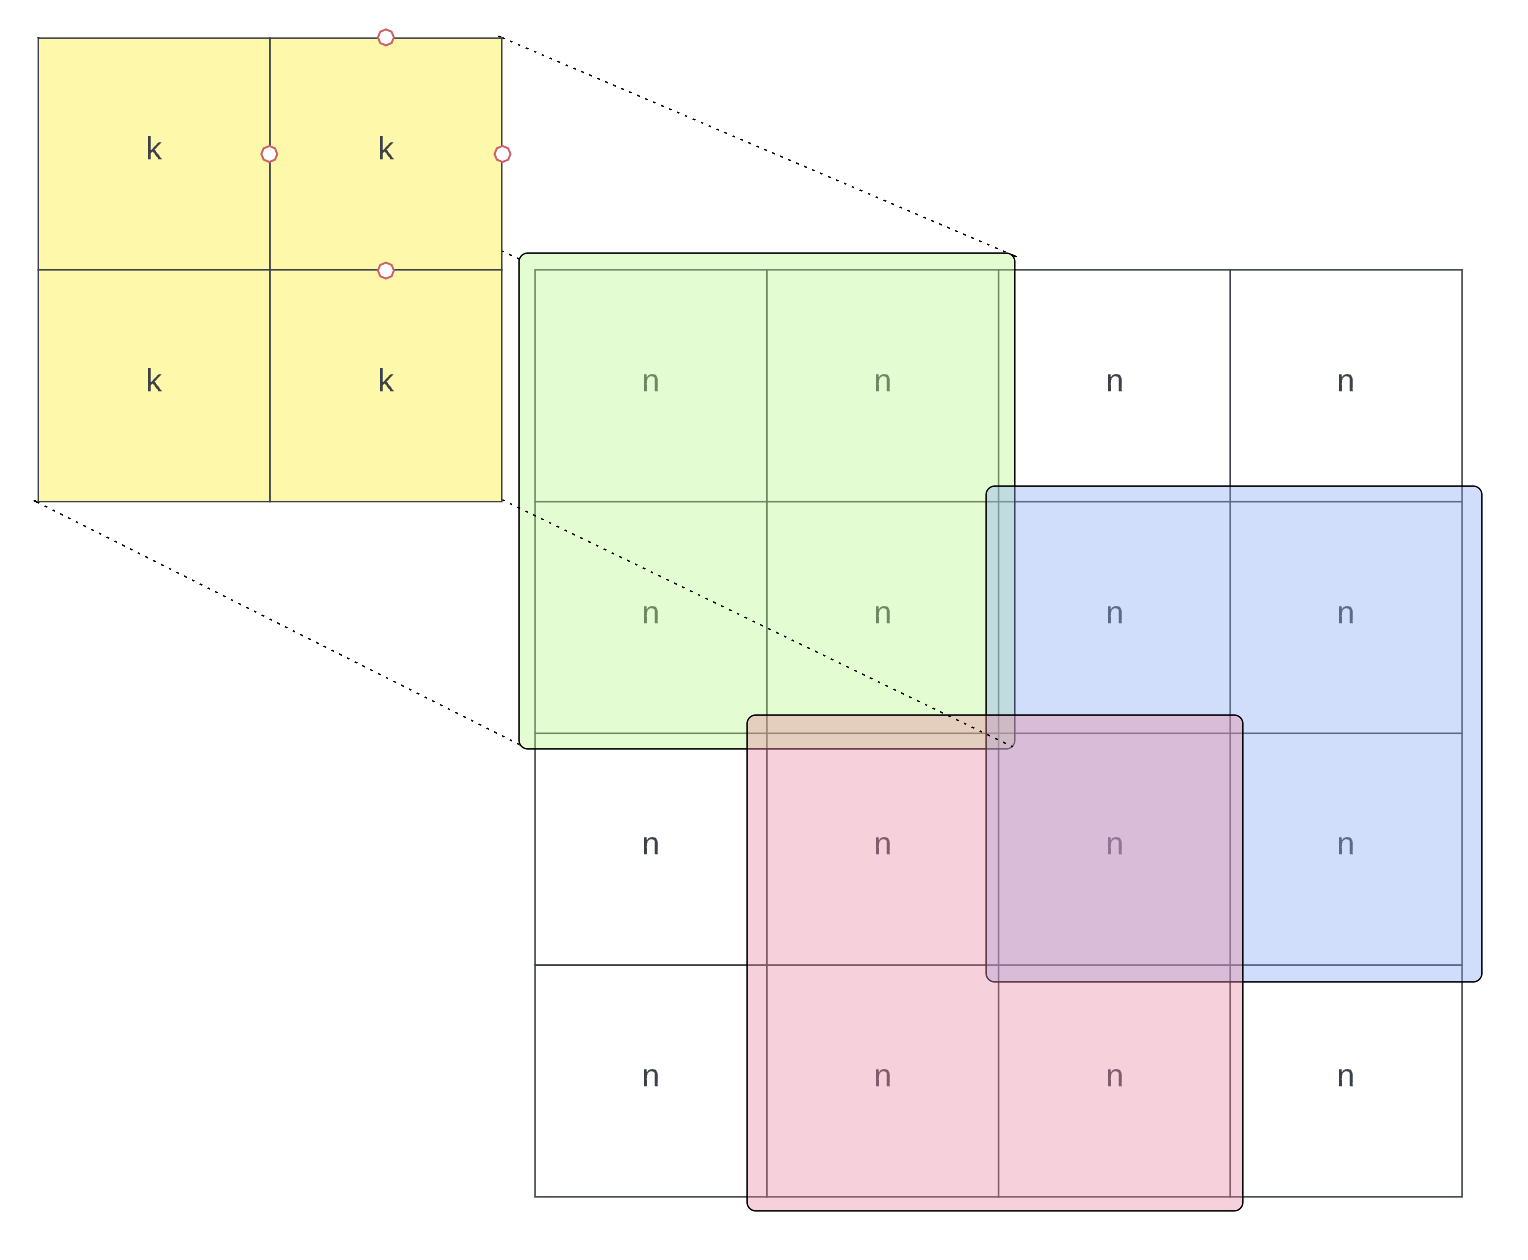
\includegraphics[width=0.8\textwidth]{images/randomScanning}
	\caption{Random scanning of the image}
	\label{fig:randomScanning}
\end{figure}

This type of convolution when used only during inference using PEMAN could drastically reduce the number of operations required and would thereby boost the speed of the structure. The tradeoff is that the accuracy of the model would be reduced.

After changing the exact same model from previous study to use random scanning during inference, the accuracy came out to be 18.78\%. This is significantly lower than previous models and is paractically not acceptable. Thus, this method needs to be explored further and researched as to which model and architecture would benefit this method the most.